%----------------------------------------------------------------------------------------
%	PACKAGES AND OTHER DOCUMENT CONFIGURATIONS
%----------------------------------------------------------------------------------------

\documentclass{article} % paper and 12pt font size
\usepackage{amsmath,amsfonts,amsthm} % Math packages
\usepackage[margin=1in]{geometry}
\usepackage[ruled,vlined]{algorithm2e}
\usepackage{graphicx}
\usepackage{float}
\usepackage{tabu}
\usepackage[parfill]{parskip}
\usepackage[labelsep=quad,indention=10pt]{subfig}
\setlength{\paperwidth}{8.5in}
\setlength{\paperheight}{11in}

%----------------------------------------------------------------------------------------
%	TITLE SECTION
%----------------------------------------------------------------------------------------

\newcommand{\horrule}[1]{\rule{\linewidth}{#1}} % Create horizontal rule command with 1 argument of height

\title{	
\normalfont \normalsize 
\textsc{University of Texas at Austin, CS 391L} \\
\horrule{0.6pt} \\[0.4cm] % Thin top horizontal rule
\huge Homework 3 - Sampling \\[0.4cm]
\large Write Up  \\
\horrule{2pt} \\[0.5cm] % Thick bottom horizontal rule
}
\author{Venketaram Ramachandran\\
vr7948 - venket@cs.utexas.edu} % Your name
\date{\normalsize\today} % Today's date or a custom date

\begin{document}

\maketitle % Print the title

%----------------
% Approach
%----------------
\section{Overview}

In this assignment, I leveraged the Metropolis algorithm to sample from a given distribution. For target distributions, I used the requested \(p(x)=0.3N(-25,10) + 0.7(20,10)\) distribution for a 1D case and the distribution \(p(x)=0.3N(\mu_1,\sigma_1)+0.7N(\mu_2,\sigma_2)\) for a 2D case, where: 
\(\mu_1=\) $\bigl(\begin{smallmatrix}
-25&-25
\end{smallmatrix} \bigr)$, 
\(\mu_2=\) $\bigl(\begin{smallmatrix}
-25&-25
\end{smallmatrix} \bigr)$, 
\(\sigma_1=\) $\bigl(\begin{smallmatrix}
100&25\\10&90
\end{smallmatrix} \bigr)$, 
\(\sigma_2=\) $\bigl(\begin{smallmatrix}
90&20\\20&90
\end{smallmatrix} \bigr)$.
The following two images depict the target distributions for the experiments below:

\begin{figure}[h]%
	\centering
    	\subfloat[1D Distribution]{%
        	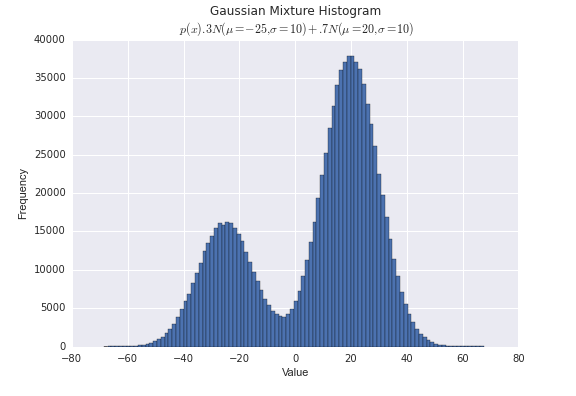
\includegraphics[width=80mm]{mixture.png}%
            \label{fig:left}%
        }\hfill%
        \subfloat[2D Distribution]{%
        	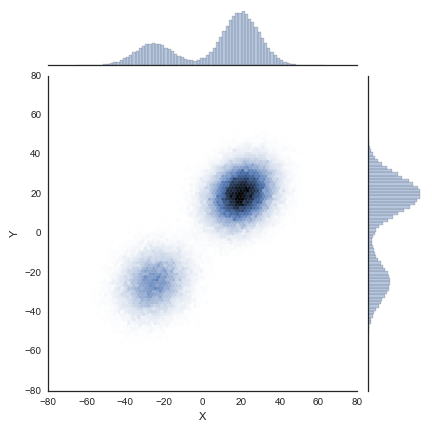
\includegraphics[width=80mm]{mixture_2d____1___0___0A___0___1___.png}%
            \label{fig:right}%
        }
    \caption{\textit{Target distributions used in the assignment}}
    \label{fig:default}
\end{figure}

In high-dimensional spaces, sampling can be an extremely expensive task.

\section{Approach}

In general, the approach that I took was exactly similar to that proposed in the Pattern Recognition and Machine Learning book and the algorithm outline described in the Berlin Humboldt University notes\footnote{http://sfb649.wiwi.hu-berlin.de/fedc\_homepage/xplore/ebooks/html/csa/node27.html} for Markov Chain Monte Carlo algorithms. For the sake of brevity, I'm not reproducing the entire algorithm here.

The only area where I differ slightly from the book and the reference page's algorithms is in the acceptance condition computation. While the overall logic is consistent with that of the references, I deal with log probabilities rather than the probability density values. This is a result of utilizing the Gaussian Mixture Model from the sk-Learn library in Python, which provides probability density values as log probabilities. Let \( x \) be the previous selection and \( x^* \) be the candidate. The modification to original condition \(min(1, \frac{p(x^*)}{p(x)})\) to use log probabilities are the following manner:

\begin{itemize}
\item If $ log(p(x^*)) > log(p(x)) $, then transition to the new state. This is effectively the bound achieved by the 1 in the min term.
\item Otherwise, retrieve the value of $ \alpha = e^{[log(p(x^*)) - log(p(x))]} $ and transition to the new state with probability $ \alpha $. This ratio is equivalent to the probability ratio. 
\item Else, stay at the same state. This is exactly the same as the original conditions.
\end{itemize}

\section{Experiments}

The following subsections describe the experiments I did, the results I received, and the observations I made. All experiments described here can be reproducible through the submitted iPython notebook, which similarly walks through cases.

\subsection{1D Distribution}

\subsubsection{Setup}

I ran the Metropolis algorithm for standard deviation values \(\sigma \in{[0.1, 10, 100, 500, 1000, 5000, 10000, 100000]}\), with an arbitrarily chosen starting point of 0. Each was run for 1,000,000 iterations.

\subsubsection{Results}

As expected, there was variability in the results produced. In some of them, the sampled distribution looked quite similar to the target distribution. Figure 2 shows the results of the above runs, while Table 1 describes the rejection rates, which is simply 1 - acceptance rate, for each case.

\begin{table*}[h]
\centering
\caption{\label{tab:widgets} \textit{Rejection Rates for various values of \(\sigma\).}}
\begin{tabu}{|c|c|c|c|c|c|c|c|c|}
\hline
\rowfont{\bfseries} \(\sigma\) & 0.1 & 10 & 100 & 500 & 1000 & 5000 & 10000 & 100000 \\\hline
Rejection Rate & 0.0038 & 0.2654 & 0.78739 & 0.95442 & 0.97691 & 0.99569 & 0.99773 & 0.9997 \\\hline
\end{tabu}
\end{table*}

\begin{figure}%
	\centering
    	\subfloat[\(\sigma=0.1\)]{%
        	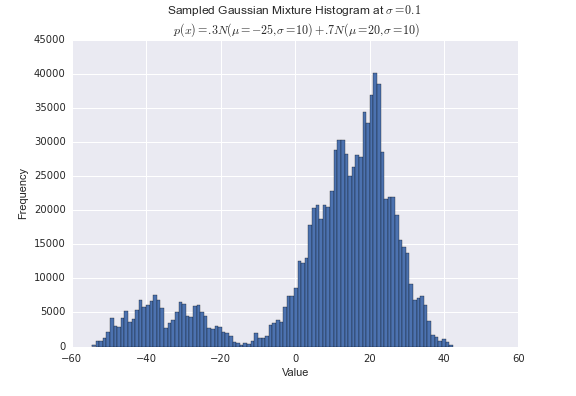
\includegraphics[width=70mm]{mixture_sampled_0_1.png}%
            \label{fig:left}%
        }\hfill%
        \subfloat[\(\sigma=10\)]{%
        	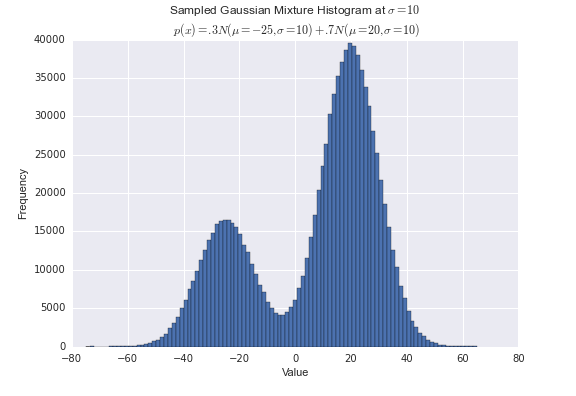
\includegraphics[width=70mm]{mixture_sampled_10.png}%
            \label{fig:left}%
        }\hfill%
        \subfloat[\(\sigma=100\)]{%
        	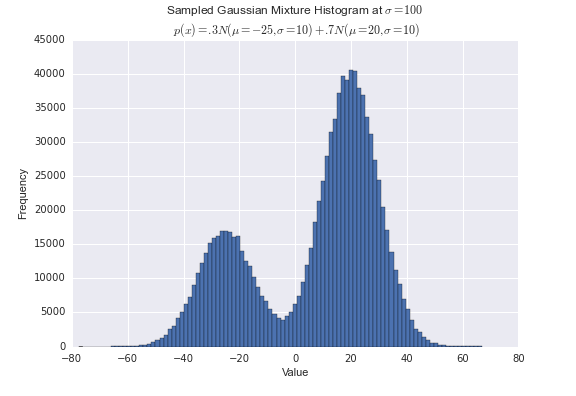
\includegraphics[width=70mm]{mixture_sampled_100.png}%
            \label{fig:right}%
        }\hfill%
        \subfloat[\(\sigma=500\)]{%
        	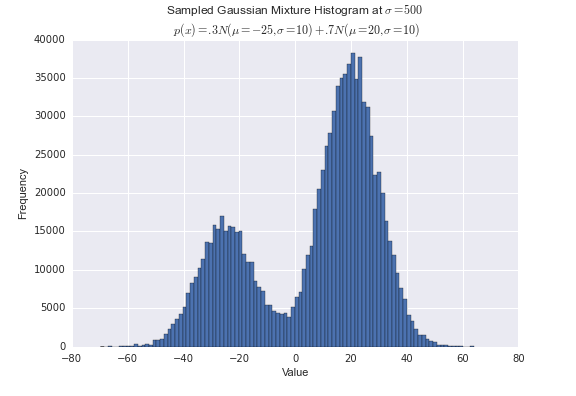
\includegraphics[width=70mm]{mixture_sampled_500.png}%
            \label{fig:right}%
        }\hfill%
        \subfloat[\(\sigma=1000\)]{%
        	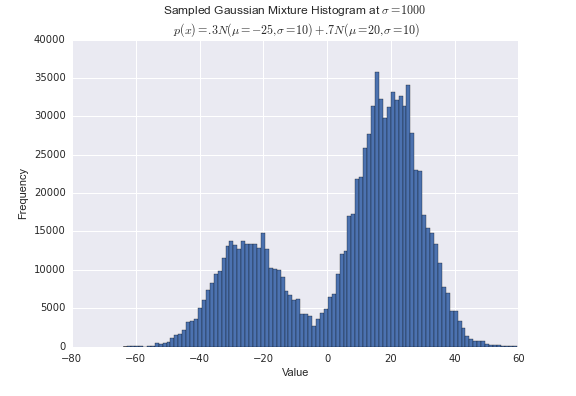
\includegraphics[width=70mm]{mixture_sampled_1000.png}%
            \label{fig:right}%
        }\hfill%
        \subfloat[\(\sigma=5000\)]{%
        	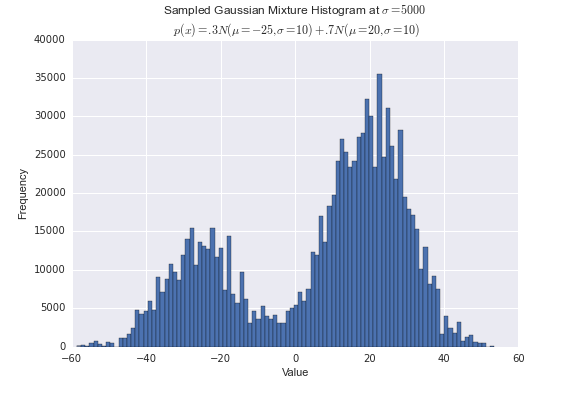
\includegraphics[width=70mm]{mixture_sampled_5000.png}%
            \label{fig:right}%
        }\hfill%
        \subfloat[\(\sigma=10000\)]{%
        	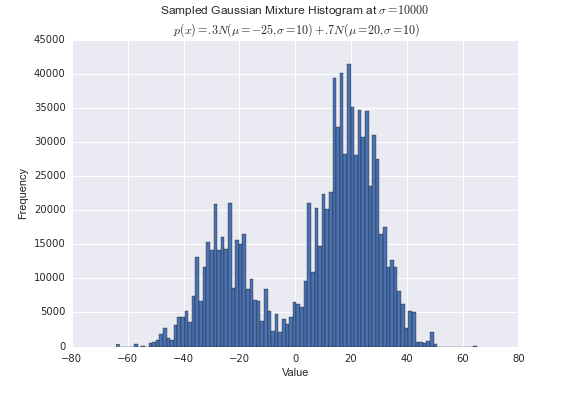
\includegraphics[width=70mm]{mixture_sampled_10000.png}%
            \label{fig:right}%
        }\hfill%
        \subfloat[\(\sigma=100000\)]{%
        	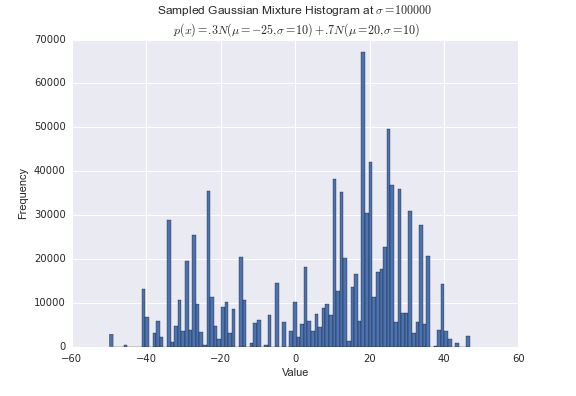
\includegraphics[width=70mm]{mixture_sampled_100000.png}%
            \label{fig:right}%
        }
    \caption{\textit{Results of sampling with Metropolis (1D case).}}
    \label{fig:default}
\end{figure}

In general, the \(\sigma\) value of 10 and 100 seemed to perform the best of the the choice of \(sigma\) used. Based on the actual graph itself, the true optimal value likely lies in between the two values. In smaller variances, there seemed to be less adherence to the actual distribution itself (i.e. the plot looked dissimilar to the target distribution plot). This was especially true in the larger \(\sigma\), where as the value of \(\sigma\) increased, the shape began to look further dissimilar.

\subsubsection{Observations}

The results observed follow closely with the sampling theory regarding the Metropolis algorithm. Specifically, if the value of \(\sigma\) is too small, then the algorithm doesn't necessarily explore very well, accepting many candidates. This is reflected in the curvature of the \(\sigma=0.1\) case. Although the general shape of the distribution is more or less present, there isn't any definition and the shape will continue likely evolving towards the expected target distribution shape. If this takes forever, this defeats the purpose of the Metropolis algorithm.

Similarly, much larger than ideal variances imply that the algorithm is too quickly and broadly exploring the space of values. This results in the problem that there will be significantly less acceptances and the nuances of the distribution will be lost. By always reaching widespread for potential values, the setup makes it unlikely for candidates to be a part of the target distribution and as a result, the overall distribution will not be captured. This is highly visible in the changes from \(\sigma=1000\) to \(\sigma=5000\) to \(\sigma=10000\) to \(\sigma=100000\).

The "sweet-spot" of this scenario was the \(\sigma=10\) case. Of the cases attempted, it seemed the most similarly shaped curve to the target distribution. For this scenario, it likely a balance between how much it facilitated exploration versus being able to traverse slowly enough to capture the nuances of the distribution. 

The concept of exploration as well as the results in Table 1 leads to an interesting observation regarding the acceptance rate. In particular, the acceptance rate can be seen as a mechanism of evaluating to what degree exploration has occurred. If the acceptance rate is near zero, this implies that nothing had been accepted and the algorithm is exploring too far. If the acceptance rate is near 1, this implies that the algorithm may not be exploring enough. In particular, we may want a mixture of acceptances and rejections. Based on Table 1, this is likely a reflection of why \(\sigma=10\) seemingly performed better than the others and provides foundation towards the hypothesis that \(\sigma\) between 10 and 100 will likely be the optimal sigma for this scenario. 

\subsection{2D Distribution}

\subsubsection{Setup}

For the 2D cases, I attempted multiple covariance matrices, \(\Sigma \in [
\bigl(\begin{smallmatrix} 1&0\\0&1 \end{smallmatrix} \bigr), \bigl(\begin{smallmatrix} 20&0\\0&20 \end{smallmatrix} \bigr), \bigl(\begin{smallmatrix} 100&0\\0&100 \end{smallmatrix} \bigr), \bigl(\begin{smallmatrix} 1000&0\\0&1000 \end{smallmatrix} \bigr), \\ \bigl(\begin{smallmatrix} 10000&0\\0&10000 \end{smallmatrix} \bigr),
\bigl(\begin{smallmatrix} 100000&0\\0&100000 \end{smallmatrix} \bigr) ]\), with an arbitrarily chosen starting point of \((0\ 0)\). I started with the identity matrix for covariance and then scaled the covariance higher to similarly inspect the impact of covariance on the sampling distribution generated. Each was run for 100,000 iterations rather than 1,000,000 iterations due to computational limitations.

\subsubsection{Results}

As before in the 1D case, there was variability in the results produced. Though no particular run exactly imitated the target distribution some came close. Figure 3 displays the results of the runs while Table 2 shows the rejection rates.

\newsavebox{\smlmat}% Box to store smallmatrix content
\savebox{\smlmat}{$\left(\begin{smallmatrix}100000&0\\0&100000\end{smallmatrix}\right)$}
\newsavebox{\smlmatt}% Box to store smallmatrix content
\savebox{\smlmatt}{$\left(\begin{smallmatrix}1&0\\0&1\end{smallmatrix}\right)$}
\newsavebox{\smlmattt}% Box to store smallmatrix content
\savebox{\smlmattt}{$\left(\begin{smallmatrix}20&0\\0&20\end{smallmatrix}\right)$}
\newsavebox{\smlmatttt}% Box to store smallmatrix content
\savebox{\smlmatttt}{$\left(\begin{smallmatrix}100&0\\0&100\end{smallmatrix}\right)$}
\newsavebox{\smlmattttt}% Box to store smallmatrix content
\savebox{\smlmattttt}{$\left(\begin{smallmatrix}1000&0\\0&1000\end{smallmatrix}\right)$}
\newsavebox{\smlmatttttt}% Box to store smallmatrix content
\savebox{\smlmatttttt}{$\left(\begin{smallmatrix}10000&0\\0&10000\end{smallmatrix}\right)$}

\begin{table*}[h]
\centering
\caption{\label{tab:widgets} \textit{Rejection Rates for various values of \(\Sigma\).}}
\begin{tabu}{|c|c|c|c|c|c|c|}
\hline
\rowfont{\bfseries} \(\Sigma\) & \usebox{\smlmatt} & \usebox{\smlmattt} & \usebox{\smlmattt} & \usebox{\smlmatttt} & \usebox{\smlmattttt} & \usebox{\smlmat} \\\hline
Rejection Rate & 0.05364 & 0.22478 & 0.46204 & 0.83044 & 0.97028 & 0.99636 \\\hline
\end{tabu}
\end{table*}

\begin{figure}%
	\centering
        \subfloat[\(\Sigma=\)\usebox{\smlmatt}]{%
        	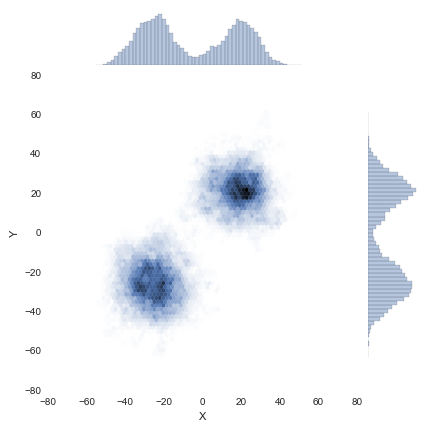
\includegraphics[width=65mm]{mixture_sampled____1___0___0A___0___1___.png}%
            \label{fig:left}%
        }\hfill%
        \subfloat[\(\Sigma=\)\usebox{\smlmattt}]{%
        	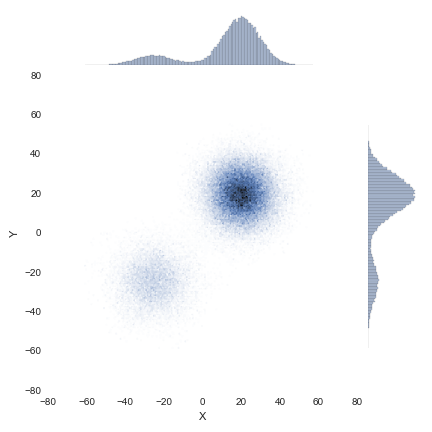
\includegraphics[width=65mm]{mixture_sampled___20__10____10__20__.png}%
            \label{fig:right}%
        }\hfill%
        \subfloat[\(\Sigma=\)\usebox{\smlmatttt}]{%
        	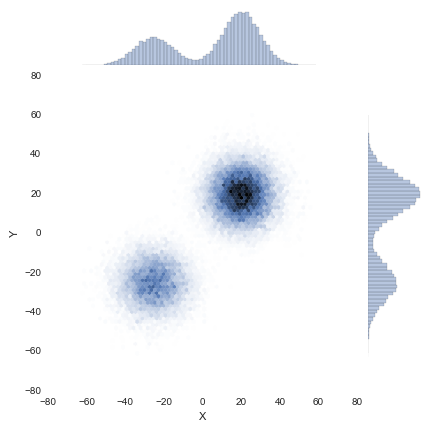
\includegraphics[width=65mm]{mixture_sampled___100__0____0__100__.png}%
            \label{fig:right}%
        }\hfill%
        \subfloat[\(\Sigma=\)\usebox{\smlmattttt}]{%
        	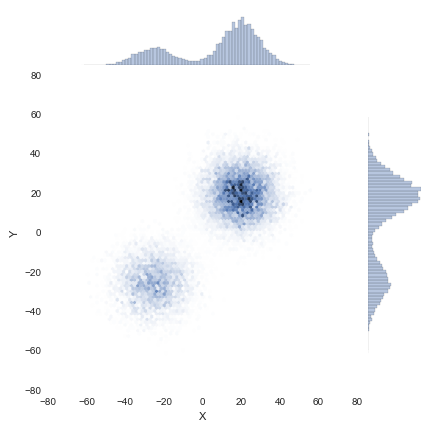
\includegraphics[width=65mm]{mixture_sampled___1000__0____0__1000__.png}%
            \label{fig:right}%
        }\hfill%
        \subfloat[\(\Sigma=\)\usebox{\smlmatttttt}]{%
        	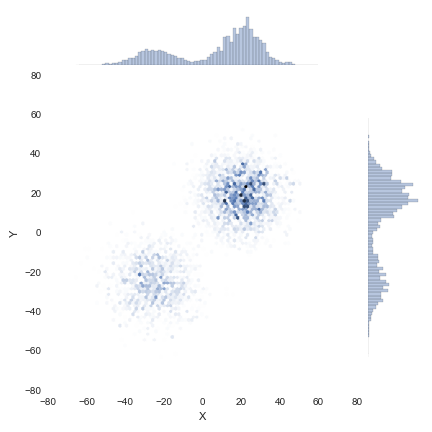
\includegraphics[width=65mm]{mixture_sampled___10000__0____0__10000__.png}%
            \label{fig:right}%
        }\hfill%
        \subfloat[\(\Sigma=\)\usebox{\smlmat}]{%
        	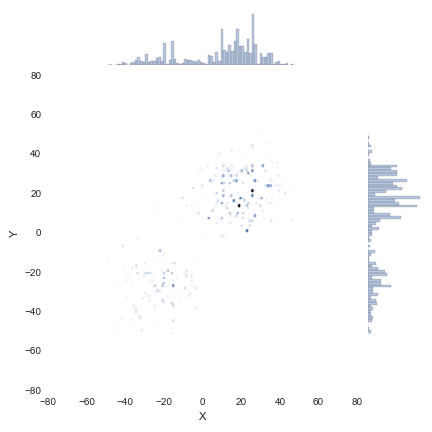
\includegraphics[width=65mm]{mixture_sampled___100000__0____0__100000__.png}%
            \label{fig:left}%
        }
    \caption{\textit{Results of sampling with Metropolis (2D case).}}
    \label{fig:default}
\end{figure}

Similar to the 1D case, there were sweet spots, where the distribution looked similar to the target distribution. In particular, the \(\Sigma =  \bigl(\begin{smallmatrix} 100&0\\0&100 \end{smallmatrix} \bigr)\) and \(\Sigma = \bigl(\begin{smallmatrix} 100&0\\0&100 \end{smallmatrix} \bigr)\) cases looked similar to the original distribution, though they were slightly off. 

\subsubsection{Observations}

The patterns observed with the 1D case is present in the 2D case as well. When the covariance is relatively low, there is a presence of extremely slow exploration. Due to that, the actual distribution's pattern is not yet fully captured. On the flipside, having an extremely high variance, as in the \(\Sigma = \bigl(\begin{smallmatrix} 100000&0\\0&100000 \end{smallmatrix} \bigr)\) case, the distribution's nuances are not fully well explored due to the fact that very little candidates are likely accepted. The \(\Sigma =  \bigl(\begin{smallmatrix} 100&0\\0&100 \end{smallmatrix} \bigr)\) and \(\Sigma = \bigl(\begin{smallmatrix} 100&0\\0&100 \end{smallmatrix} \bigr)\) cases both seemed closer to the actual distribution because they likely both explored and picked up the distribution nuances. The notion is reinforced by the rejection rates in Table 2, which shows that both cases had a good mix of acceptance and rejection, indicating a mixture of exploration and picking up the distribution nuances.

Figuring out a proper standard deviation in the 1D case was a non-trivial problem. It is even more so given the extra dimension in the 2D case. Of the variances that I've chosen, none are truly perfect. In general, based on literature across the web, selecting an appropriate covariance as well as a proposal distribution seems to be an art that requires intuition and/or a lot of trial-and-error. 

\section{Metropolis-Hastings}

I extended the homework prompt, which required implementing the Metropolis Algorithm, to also implement the Metropolis-Hastings algorithm. The generalization of the algorithm only required the addition of the extra term accounting for the case if the proposal distribution is no longer a symmetric function of its arguments. Figure 4 displays the results from the Metropolis-Hastings on a selection of the cases from the 1D experiments while Figure 5 displays the results from the Metropolis-Hastings algorithm on a selection of the cases from the 2D experiments. Please refer to the iPython notebook for all cases reproduced. 

\begin{figure}%
	\centering
        \subfloat[\(\sigma=10\)]{%
        	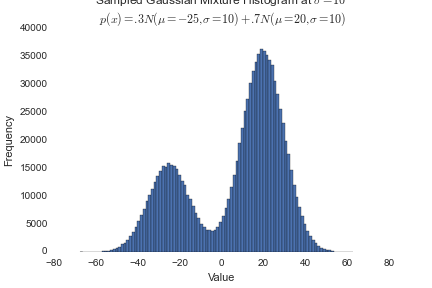
\includegraphics[width=70mm]{mixture_sampled_hastings_10.png}%
            \label{fig:left}%
        }\hfill%
        \subfloat[\(\sigma=100\)]{%
        	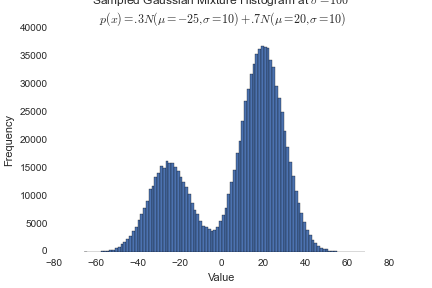
\includegraphics[width=70mm]{mixture_sampled_hastings_100.png}%
            \label{fig:right}%
        }\hfill%
        \subfloat[\(\sigma=1000\)]{%
        	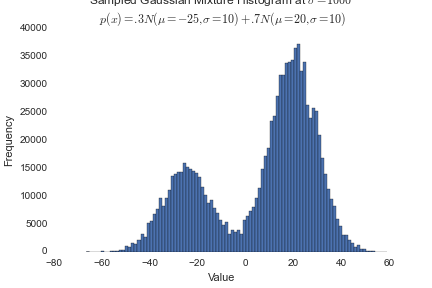
\includegraphics[width=70mm]{mixture_sampled_hastings_1000.png}%
            \label{fig:right}%
        }\hfill%
        \subfloat[\(\sigma=10000\)]{%
        	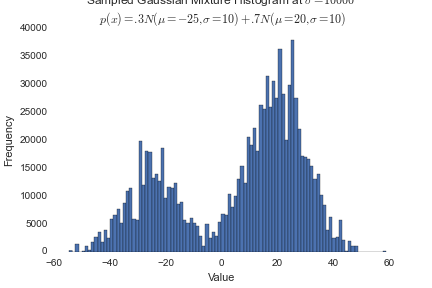
\includegraphics[width=70mm]{mixture_sampled_hastings_10000.png}%
            \label{fig:right}%
        }
    \caption{\textit{Results of sampling with Metropolis-Hastings (1D case).}}
    \label{fig:default}
\end{figure}


\begin{figure}%
	\centering
        \subfloat[\(\Sigma=\)\usebox{\smlmattt}]{%
        	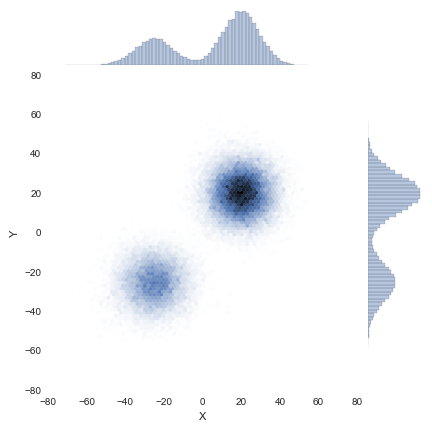
\includegraphics[width=65mm]{mixture_sampled_hastings___20__0____0__20__.png}%
            \label{fig:right}%
        }\hfill%
        \subfloat[\(\Sigma=\)\usebox{\smlmatttt}]{%
        	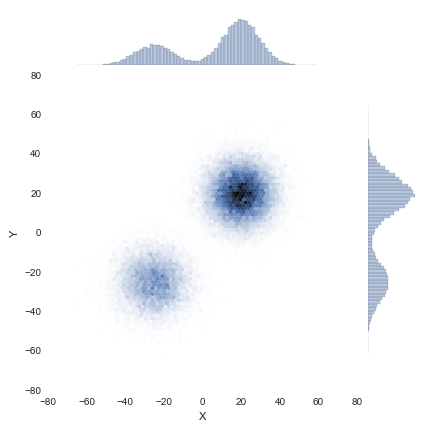
\includegraphics[width=65mm]{mixture_sampled_hastings___100__0____0__100__.png}%
            \label{fig:right}%
        }\hfill%
        \subfloat[\(\Sigma=\)\usebox{\smlmattttt}]{%
        	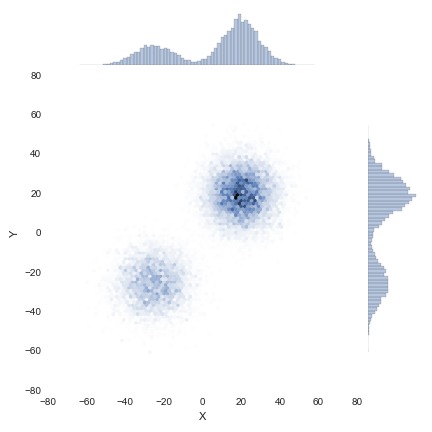
\includegraphics[width=65mm]{mixture_sampled_hastings___1000__0____0__1000__.png}%
            \label{fig:right}%
        }\hfill%
        \subfloat[\(\Sigma=\)\usebox{\smlmatttttt}]{%
        	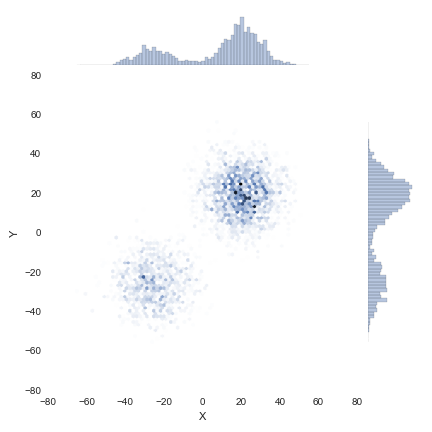
\includegraphics[width=65mm]{mixture_sampled_hastings___10000__0____0__10000__.png}%
            \label{fig:right}%
        }
    \caption{\textit{Results of sampling with Metropolis-Hastings (2D case).}}
    \label{fig:default}
\end{figure}

Given that the above distributions were all symmetric, as expected, the distributions created through the Metropolis-Hastings algorithm are quite similar. Attempting to use other covariance combinations (i.e. not  scaled versions of the identity matrix) did not provide any significantly better results (i.e. please check the iPython notebook). This scenario illustrates again that choosing a proposal distribution and the appropriate variance is a non-trivial task.

\section{Concluding Notes}

In future work, I would be interested in exploring adaptive variations of Metropolis-Hastings algorithm. Being able to tune the proposal distribution, which with the exception of centering around the mean of a sample, is fairly static might provide areas for optimization. I would also be interested in leveraging the acceptance rates, which provide a fair bit of context in helping analyze the degree in which exploration is occurring, to investigate adaptive techniques.

\end{document}
